% Options for packages loaded elsewhere
\PassOptionsToPackage{unicode}{hyperref}
\PassOptionsToPackage{hyphens}{url}
%
\documentclass[
]{article}
\usepackage{amsmath,amssymb}
\usepackage{lmodern}
\usepackage{iftex}
\ifPDFTeX
  \usepackage[T1]{fontenc}
  \usepackage[utf8]{inputenc}
  \usepackage{textcomp} % provide euro and other symbols
\else % if luatex or xetex
  \usepackage{unicode-math}
  \defaultfontfeatures{Scale=MatchLowercase}
  \defaultfontfeatures[\rmfamily]{Ligatures=TeX,Scale=1}
\fi
% Use upquote if available, for straight quotes in verbatim environments
\IfFileExists{upquote.sty}{\usepackage{upquote}}{}
\IfFileExists{microtype.sty}{% use microtype if available
  \usepackage[]{microtype}
  \UseMicrotypeSet[protrusion]{basicmath} % disable protrusion for tt fonts
}{}
\makeatletter
\@ifundefined{KOMAClassName}{% if non-KOMA class
  \IfFileExists{parskip.sty}{%
    \usepackage{parskip}
  }{% else
    \setlength{\parindent}{0pt}
    \setlength{\parskip}{6pt plus 2pt minus 1pt}}
}{% if KOMA class
  \KOMAoptions{parskip=half}}
\makeatother
\usepackage{xcolor}
\usepackage[margin=1in]{geometry}
\usepackage{graphicx}
\makeatletter
\def\maxwidth{\ifdim\Gin@nat@width>\linewidth\linewidth\else\Gin@nat@width\fi}
\def\maxheight{\ifdim\Gin@nat@height>\textheight\textheight\else\Gin@nat@height\fi}
\makeatother
% Scale images if necessary, so that they will not overflow the page
% margins by default, and it is still possible to overwrite the defaults
% using explicit options in \includegraphics[width, height, ...]{}
\setkeys{Gin}{width=\maxwidth,height=\maxheight,keepaspectratio}
% Set default figure placement to htbp
\makeatletter
\def\fps@figure{htbp}
\makeatother
\setlength{\emergencystretch}{3em} % prevent overfull lines
\providecommand{\tightlist}{%
  \setlength{\itemsep}{0pt}\setlength{\parskip}{0pt}}
\setcounter{secnumdepth}{-\maxdimen} % remove section numbering
\usepackage{booktabs}
\usepackage{longtable}
\usepackage{array}
\usepackage{multirow}
\usepackage{wrapfig}
\usepackage{float}
\usepackage{colortbl}
\usepackage{pdflscape}
\usepackage{tabu}
\usepackage{threeparttable}
\usepackage{threeparttablex}
\usepackage[normalem]{ulem}
\usepackage{makecell}
\usepackage{xcolor}
\ifLuaTeX
  \usepackage{selnolig}  % disable illegal ligatures
\fi
\IfFileExists{bookmark.sty}{\usepackage{bookmark}}{\usepackage{hyperref}}
\IfFileExists{xurl.sty}{\usepackage{xurl}}{} % add URL line breaks if available
\urlstyle{same} % disable monospaced font for URLs
\hypersetup{
  pdftitle={EDA},
  pdfauthor={javier saavedra},
  hidelinks,
  pdfcreator={LaTeX via pandoc}}

\title{EDA}
\author{javier saavedra}
\date{9/29/2022}

\begin{document}
\maketitle

En el presente informe realizaremos un analisis exploratorio a nuestra
base de datos ``accelerometer''. Esta base de datos consiste en valores
recopilados a traves de un acelerometro montado en un aspa propulsada
por un motor, respecto al aspa tenemos 3 variantes, las cuales se
diferencian por pesos dispuestos de maneras distintas para generar 3
escenarios de vibraciones distintas para analizar, estos datos
transcurren dependiendo de las revoluciones de giro del motor( RPM).

los casos a observar son los siguientes

\begin{itemize}
\item Rojo: Configuración normal dos piezas de peso colocadas en palas vecinas
\item Azul: Configuración perpendicular dos piezas de peso colocadas sobre palas que forman un ángulo de 90 grados
\item Verde: Configuración opuesta dos piezas de peso colocadas en palas opuestas
\end{itemize}

Un vistazo a los datos.

\begin{verbatim}
##    Aspa  RPM     X      Y      z
## 1  rojo  380 1.004  0.090 -0.125
## 2  rojo 1140 1.168  0.688 -0.191
## 3  rojo 1900 0.582  0.871  0.621
## 4  azul  380 0.992 -0.008 -0.129
## 5  azul 1140 0.996 -0.289 -0.340
## 6  azul 1900 2.418 -1.172 -0.523
## 7 verde  380 0.996  0.098 -0.113
## 8 verde 1140 0.949  0.004 -0.121
## 9 verde 1900 0.949 -0.125 -0.125
\end{verbatim}

Como podemos imaginar, los valores corresponden a la tasa de cambio de
la velocidad de giro en 3 ejes, estos valores nos ayudan a detectar las
vibracion en el aspa y como estas varian al aumentar las rpm, es por
esto que un analisis exploratorio no ayudara a detectar comportamientos,
tendencias y estadisticas utiles para los fines del estudio
correspondiente. \newpage

\hypertarget{analisis-de-dispersion}{%
\subsection{analisis de dispersion}\label{analisis-de-dispersion}}

Aqui podemos observar la distribucion de los datos segun el aspa. se
puede notar por la transparencia de los puntos donde hay mayor
concentracion de puntos y la variacion por la distancia vertical entre
los puntos

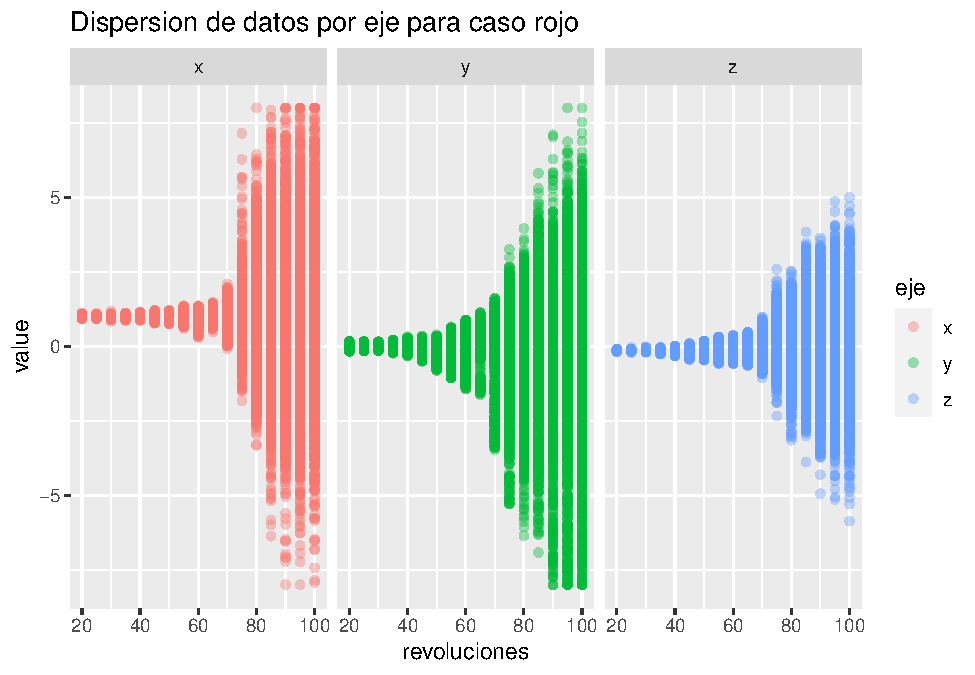
\includegraphics{EDA_files/figure-latex/unnamed-chunk-3-1.pdf}
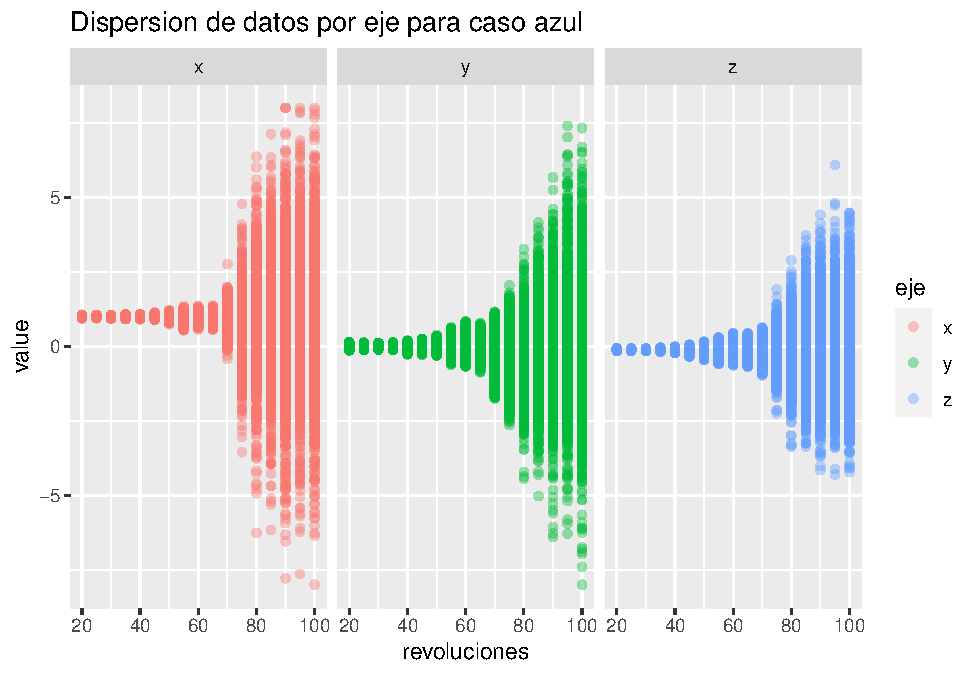
\includegraphics{EDA_files/figure-latex/unnamed-chunk-3-2.pdf}
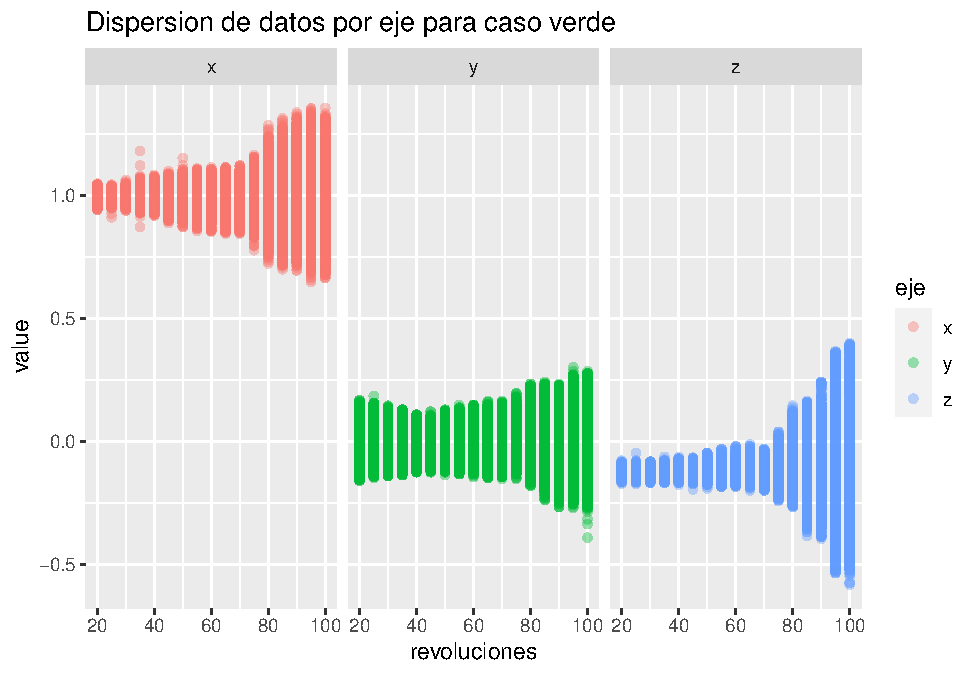
\includegraphics{EDA_files/figure-latex/unnamed-chunk-3-3.pdf}

\newpage

\hypertarget{medidas-de-tendencia-central}{%
\subsection{medidas de tendencia
central}\label{medidas-de-tendencia-central}}

Ahora observamos algunas estadisticas de interes

\begin{table}

\caption{\label{tab:unnamed-chunk-4}Summary Statistics}
\centering
\begin{tabular}[t]{llllll}
\toprule
Variable & NotNA & Mean & Var & Min & Max\\
\midrule
wconfid: rojo &  &  &  &  & \\
x & 51000 & 1 & 1.167 & -8 & 7.996\\
y & 51000 & -0.004 & 1.168 & -8 & 7.996\\
z & 51000 & -0.122 & 0.477 & -5.867 & 4.992\\
wconfid: azul &  &  &  &  & \\
\addlinespace
x & 51000 & 0.998 & 0.624 & -8 & 7.996\\
y & 51000 & 0.014 & 0.479 & -8 & 7.391\\
z & 51000 & -0.112 & 0.317 & -4.305 & 6.086\\
wconfid: verde &  &  &  &  & \\
x & 51000 & 0.989 & 0.006 & 0.648 & 1.355\\
\addlinespace
y & 51000 & 0.006 & 0.007 & -0.391 & 0.301\\
z & 51000 & -0.119 & 0.008 & -0.582 & 0.398\\
\bottomrule
\end{tabular}
\end{table}

\hypertarget{que-podemos-decir-de-los-datos}{%
\subsubsection{¿Que podemos decir de los
datos?}\label{que-podemos-decir-de-los-datos}}

A simple vista notamos que el aspa de caso verde tiene la menor
variabilidad de los 3 casos, por otro lado vemos que el minimo y maximo
en los casos rojo y azul son identicos, esto no implica que tengan el
mismo comportamienta, como vimos en los graficos anteriores, los datos
del caso azul se encuentran mas concentrados en la media por lo cual las
vibraciones serian menos significativas. Observamos que los datos de los
ejes no covarian entre si.

Sin embargo, el analisis nos causa muchas preguntas principalmente sobre
informacion del motor para hacer una interpretacion de los datos, a su
vez no sabemos en que eje y sentido gira el aspa, lo cual nos ayudaria a
dar distinta importancia a los valores de cada eje.

Como conclusion mencionamos la baja variabilidad de los datos del caso
verde lo cual supondria un mejor comportamiento del aspa independiente
del contexto en el que se estudie, considerando que estos datos fueron
utilizados para predecir la duracion de vida de un motor, pensamos que
el caso verde otorgaria la mayor vida al motor.

\end{document}
